% v2-acmsmall-sample.tex, dated March 6 2012
% This is a sample file for ACM small trim journals
%
% Compilation using 'acmsmall.cls' - version 1.3 (March 2012), Aptara Inc.
% (c) 2010 Association for Computing Machinery (ACM)
%
% Questions/Suggestions/Feedback should be addressed to => "acmtexsupport@aptaracorp.com".
% Users can also go through the FAQs available on the journal's submission webpage.
%
% Steps to compile: latex, bibtex, latex latex
%
% For tracking purposes => this is v1.3 - March 2012

\documentclass[prodmode,acmtecs]{acmsmall} % Aptara syntax

% Package to generate and customize Algorithm as per ACM style
\usepackage[linesnumbered]{algorithm2e}
\usepackage{fancyvrb}
\usepackage{paralist}
\usepackage{amsmath}
\usepackage{amssymb}
\usepackage{subfig}
\renewcommand{\algorithmcfname}{ALGORITHM}
\newenvironment{algo}{%
\renewenvironment{algocf}[1][h]{}{}%
\algorithm
}{%
\endalgorithm
}
\SetAlFnt{\small}
\SetAlCapFnt{\small}
\SetAlCapNameFnt{\small}
\SetAlCapHSkip{0pt}
\IncMargin{-\parindent}
\newsavebox{\verbbox}
\newsavebox{\verbboxx}
\newsavebox{\eone}
\newsavebox{\etwo}

% Metadata Information
\acmVolume{}
\acmNumber{}
\acmArticle{}
\acmYear{2014}
\acmMonth{11}

% Document starts
\begin{document}

% Page heads
\markboth{A. Malik et al.}{Compiler assisted memory model for hard real-time safety-critical
  systems}

% Title portion
\title{Compiler assisted memory model for hard real-time safety-critical
  systems}
\author{Avinash Malik
  \affil{University of Auckland}
  HeeJong Park
  \affil{University of Auckland}
  Muhammad Nadeem
  \affil{University of Auckland}
  Zoran Salcic
  \affil{University of Auckland}
}
% NOTE! Affiliations placed here should be for the institution where the
%       BULK of the research was done. If the author has gone to a new
%       institution, before publication, the (above) affiliation should NOT be changed.
%       The authors 'current' address may be given in the "Author's addresses:" block (below).
%       So for example, Mr. Abdelzaher, the bulk of the research was done at UIUC, and he is
%       currently affiliated with NASA.

\begin{abstract}
\end{abstract}

\category{}{}{}

\terms{Compiler, Static Analysis, WCET, SystemJ, Garbage Collection}

\keywords{Wireless sensor networks, media access control,
multi-channel, radio interference, time synchronization}

\acmformat{}
% At a minimum you need to supply the author names, year and a title.
% IMPORTANT:
% Full first names whenever they are known, surname last, followed by a period.
% In the case of two authors, 'and' is placed between them.
% In the case of three or more authors, the serial comma is used, that is, all author names
% except the last one but including the penultimate author's name are followed by a comma,
% and then 'and' is placed before the final author's name.
% If only first and middle initials are known, then each initial
% is followed by a period and they are separated by a space.
% The remaining information (journal title, volume, article number, date, etc.) is 'auto-generated'.

\begin{bottomstuff}

Author's addresses: 
Department of Electrical and Computer Engineering,
University of Auckland,
New Zealand
\end{bottomstuff}

\maketitle


\section{Introduction}
\label{sec:introduction}

With the advent of the Internet of Things (IoT) paradigm, the line
between embedded real-time computing and standard desktop computing is
blurring. As more sensors and actuators are connected to embedded
devices, the software code bases controlling these devices is only
predicted to grow in complexity. In order to manage this inherent
complexity, managed programming languages such as Java are being
considered even for safety-critical and real-time systems. There are two
main requirements that need to be satisfied when considering real-time
and safety-critical systems: (1) respecting environment specified space
and time bounds and (2) guaranteeing functional correctness. Both these
aspects have been studied in the research literature quite extensively
for managed languages, especially
Java~\cite{khav00,pizlo2008study,scj2013}.

For any given real-time system, \textit{Worst Case Execution Time}
(WCET) of a task should be statically known so that one or more of such
tasks can be scheduled to meet their individual
deadlines~\cite{wilhelm08}. Computing WCET of a task programmed in a
non-managed language such as `C' is a non-trivial task since detailed
knowledge of hardware and interaction of the task on this hardware needs
to be known a-priori. Managed languages need a runtime environment with
\textit{Just In Time} (JIT) compilation, which exacerbates the problem
of computing the WCET of task programmed in a managed language to such
an extent as to render it unfeasible. In order to skirt this problem,
researches (both academic and commercial) either perform ahead of time
compilation of their Java
programs~\cite{kalibera2011scheduling,pizlo2010schism} or use hardware
implemented Java virtual machines~\cite{msch05}. In either case, the JIT
compilation interference is no longer a problem in determining the WCET
of the task, instead the main challenge is now to reconcile the garbage
collection (or more generally memory allocation and garbage collection,
both) inherent to a managed language within the WCET static analysis
framework.

Many approaches to \textit{Real-time Garbage Collection} (RTGC) have
been proposed, a good survey of RTGCs can be found
in~\citeyear{pizlo2008study}. There are multiple requirements that a
RTGC needs to satisfy. From the perspective of the real-time task the
main requirement is that: (1) the maximum blocking time for a GC should
be bounded and (2) the number of \textit{times} a task may be
interrupted by the GC should be bounded. From the perspective of the GC
itself, one needs to statically guarantee that enough memory is
available to keep pace with the memory allocations demanded by the
real-time task.

There are two principle approaches to integrating RTGCs within a
real-time framework. The first approach pioneered by
Henriksson~\cite{henriksson1998scheduling} requires one to schedule the
GC real-time task as the lowest priority thread in slack time -- time
between completion of a task and its deadline to \textit{incrementally}
collect garbage. The second approach is to use a periodically running GC
as the highest priority task that preempts a real-time task and runs for
a statically determined amount of time~\cite{bacon2003real} again
incrementally collecting garbage. Both approaches require a preemptable
real-time system. In the first approach the GC task might be preempted
by a higher priority real-time task or an asynchronous event. In the
second approach real-time tasks themselves need to be preempted by the
GC task. This need for preemptability has two drastic consequences: (1)
every access to heap allocated object needs to be guarded by read and
write barriers, thereby increasing time for every data access and also
memory allocation itself, which in turn increases the task's WCET. (2)
Automated functional verification of priority preemptive multi-tasking
model via approaches such as model-checking~\cite{clarke-book00,khav00}
is known to exacerbate the exponential state space explosion problem
thereby making it unfeasible to automatically verify such systems for
functional correctness.

The question then becomes: \textit{is programming real-time
  safety-critical systems using a manged language just impractical?}
One would think so, considering that the latest specification of safety
critical java does not include any form of GC~\cite{scj2013}. But still
proposes a priority preemptive multi-tasking model for safety critical
system design.

In this paper we argue that a well thought out programming model along
with compiler assisted memory management is not only a practical, but
also an efficient approach to programming real-time and safety-critical
systems using managed languages.

The most important requirement is that the programming model of the
managed language be formally verifiable or at least not be proactively
hostile to formal verification. In our opinion a system that meets all
its real-time deadlines, but is functionally incorrect is of little
use. Hence, we prioritize functional correctness over real-time
guarantees, although at the end both need to be satisfied. In order to
adhere to this requirement we consider languages (within the real-time
community) based on formal semantics that can be used for automated
formal verification. Synchronous languages such as
Esterel~\cite{gber931}, Lustre~\cite{nhal91}, Signal~\cite{pgue91} and
\textit{Globally Asynchronous Locally Synchronous} (GALS) languages such
as SystemJ~\cite{amal10} have been used to design large real-time and
safety-critical systems~\cite{bouali1998xeve,ParkMNS14,LiMS14}. All
these languages are not only based on formal mathematical semantics, but
are also designed to be amenable to automated formal
verification. Especially imperative languages Esterel and its derivation
SystemJ have been designed to reduce the state space explosion problem
exhibited during formal verification, by adhering to a very strict
programmer specified state demarcation approach. The programming model
for these languages can be described as follows: a synchronous program
is quiescent until one or more events occur from the environment. Upon
detecting the event, the synchronous program \textit{reacts}
\textit{instantaneously} in zero logical time to respond to these inputs
and becomes quiescent until the next input(s) arrive(s). The start and
end of this reaction transition demarcate states of the program -- note
that internal data changes do not lead to change in the program state
thereby reducing the state space explosion problem. Furthermore, the
reaction being logically in zero-time is by definition \textit{atomic}
and always faster than the incoming input events, thereby guaranteeing
that none of the incoming events are missed. In reality the reaction
does take sometime, all one needs to do is find out the \textit{Worst
  Case Reaction Time} (WCRT) of any given synchronous program. This WCRT
value determines the inter-arrival time for input events from the
environment.

Many techniques exist for computing WCRT values for synchronous programs
providing support for data-computation via a non-managed language
(primarily `C'). A good review is available in~\cite{wilhelm08}. We are
interested in WCRT analysis of synchronous programs that support data
computation via managed-languages like Java. The SystemJ~\cite{amal10}
language provides the synchronous programming model as a subset along
with Java driven data-computations, thereby mixing synchronous
\textit{Model of Computation} (MoC) with a managed-language runtime
environment. WCRT computation techniques have been developed for
SystemJ~\cite{LiMS14}, but the authors do not state anything about the
integration of the GC within this WCRT framework.

The main \textbf{contribution} of this paper is to present a new memory
model that is amicable to static WCRT analysis of synchronous programs
intertwined with managed runtime environments for data-support. More
concretely our contributions can be refined as follows:

\begin{itemize}
\item \textit{Programming model inspired memory organization}: In this
  paper we present a new memory organization/model for Java and
  accompanying static WCRT analysis based on the SystemJ MoC.
\item \textit{Compiler supported memory allocation}: We next present the
  compiler transformations that are needed to statically guarantee the
  \textit{Worst Case Memory Consumption} (WCMC) and \textit{allocation}.
\item \textit{Extensive benchmarks}: Finally, we provide extensive
  benchmarks comparing the proposed memory model vs. the state of the
  art RTGC approach to real-time system design.
\end{itemize}

The rest of the paper....

\section{Preliminaries}
\label{sec:preliminaries}

Before we present the key contributions of the paper, we dedicate this
section to describe the preliminary information needed by the reader.

\subsection{The SystemJ programming language}
\label{sec:syst-progr-lang}

SystemJ~\cite{amal10} extends the Java language by introducing both
synchronous and asynchronous concurrency. SystemJ integrates the
synchronous essence of Esterel~\cite{berry92} language and the
asynchronous concurrency of \textit{Communicating Sequential Processes}
(CSP)~\cite{choa78}. SystemJ is grounded on delicate and rigorous
mathematical semantics and thus is amenable to formal verification. On
the top level, a SystemJ program comprises a set of clock-domains (CDs)
executing asynchronously. Each clock-domain is a composition of one or
more synchronous parallel reactions, which are executed in lock-step
with one logical tick of the clock-domain. Reactions within the same
clock-domain exploit synchronous broadcast mechanism on signals to
communicate with each other. Reactions can themselves be composed of
more synchronous parallel reactions, thereby forming a
hierarchy. Finally, every reaction in the clock-domain communicates with
the environment through a set of interface input and output signals. At
the beginning of each clock-domain tick the input signals are captured,
a reaction function processes these input signals and emits outputs
signals. These output signals are presented to the environment at the
end of the clock-domain tick. Inter-clock-domain communication is
achieved by implementing CSP style rendezvous mechanism through
point-to-point unidirectional channels. A complete list of SystemJ
kernel statements is shown in Figure~\ref{fig:1}. In this work we are
only interested in the synchronous subset of SystemJ.

\begin{figure}[t!]
  \centering
  \[
  \begin{array}[h!]{|c|c|}
    \hline
    \mathbf{noop}  & \mathrm{do\ nothing}\\
    \hline
    \mathbf{pause}  & \mathrm{complete\ a\ logical\ tick}\\
    \hline
    \mathbf{[input] [output] [type] signal\ \sigma} &  \mathrm{declare\ signal\ \sigma} \\
    \hline
    \mathbf{emit\ \sigma [value]} &  \mathrm{broadcast\ signal\ \sigma} \\
    \hline
    \mathbf{abort\ (\sigma)\ s} &  \mathrm{preempt\ statement\ s\ if\ \sigma\ is\ true} \\
    \hline
    \mathbf{suspend\ (\sigma)\ s} &  \mathrm{suspend\ statement\ s\ for\
      one\ tick\ if\ \sigma\ is\ true} \\
    \hline
    \mathbf{present\ (\sigma)\ s1\ else\ s2} &  \mathrm{do\ s1\ if\
      \sigma\ is\ true\ else\ do\ s2} \\
    \hline
    \mathbf{s1;s2} &  \mathrm{do\ s1\ and\ then\ s2} \\
    \hline
    \mathbf{s1||s2} &  \mathrm{do\ s1\ and\ s2\ in\ lockstep\ parallel} \\
    \hline
    \mathbf{while(true)\ s} &  \mathrm{do\ s\ forever} \\
    \hline
    \mathbf{jterm} &  \mathrm{Java\ data\ term} \\
    \hline
  \end{array}
  \]
  \caption{Syntax of the synchronous subset of the SystemJ language}
  \label{fig:1}
\end{figure}

Signals are the primary means of communication between reactions of a
clock-domain and between a clock-domain and its environment. A signal in
SystemJ can be typed or untyped. Every untyped signal in SystemJ is
called a pure signal and only consists of a Boolean status, which can be
set to \texttt{true} or \texttt{false} via signal emission. A typed
signal is called a valued signal, and consists of a value (of any Java
data-type) in conjunction to the status. The value of a typed signal can
also be set optionally via the $\mathbf{emit}$ statement. Once emitted
the status of a signal is \texttt{true} only for a single tick, but the
value of a signal is persistent over ticks. Emission of a signal
broadcasts is across all reactions within the clock-domain. Moreover,
the change in status and value of the signal, upon emission, is only
visible in the next tick to other reactions.

SystemJ provides mechanism to describe reactivity via statements such as
$\mathbf{present}$, $\mathbf{abort}$, and $\mathbf{suspend}$, that
change the control-flow of a SystemJ program depending upon signal
statuses. The control-flow of a program can also be altered via standard
Java conditional constructs. Synchronous (lock-step) parallel execution
of reactions within a SystemJ program is capture using the synchronous
parallel ($||$) operator~\footnote{Standard Java threading model is not
  allowed within SystemJ, instead synchronous and asynchronous
  parallelism needs to be used.}. Furthermore, shared variable
communication between synchronous parallel reactions is not allowed in
SystemJ. The shared memory communication model is replaced by the signal
emission (broadcast) based communication mechanism. State boundaries are
demarcated explicitly by programmers using the $\mathbf{pause}$
construct. Finally, there are two types of loops in SystemJ: temporal,
consisting of a $\mathbf{pause}$ statement, loops that execute for ever
and bounded data-loops like in standard programming languages.

\subsection{The real-time execution architecture}
\label{sec:real-time-execution}

Every static WCRT analysis technique needs intimate knowledge of the
hardware that executes the program. For our purpose we choose a
multi-core real-time predictable execution platform called
\textit{Tandem-Java Optimized Processor}
(TP-JOP)~\cite{DBLP:journals/tecs/SalcicM13,nadeem2011rjop}. There are
two main reasons we chose this processor architecture: (1) efficiency --
it has been shown previously that the TP-JOP processor architecture is
much more efficient for executing SystemJ programs compared to general
purpose Java processors~\cite{ParkMNS14} and (2) there already exists
tools for statically estimating tight WCRT bounds for synchronous
SystemJ programs on the TP-JOP architecture~\cite{LiMS14}.

\begin{figure}[t!]
  \centering
  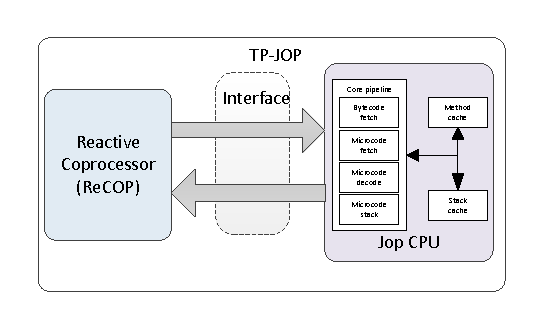
\includegraphics[scale=1.2]{tpjop}
  \caption{Overview of the TP-JOP architecture}
  \label{fig:3}
\end{figure}

Figure~\ref{fig:3} givess an overview of the TP-JOP architecture. The
architecture consists of two time predictable cores. The first core is
termed \textit{Reactive Co-processor} (ReCOP) that executes the control
flow instructions of a SystemJ program. The Java data computations are
dispatched to the JOP core on a as needed basis by the ReCOP. ReCOP has
a multi-cycle data-path, and each native ReCOP instruction is executed
in 3 clock cycles. ReCOP core uses a single small private memory for
both: data and program.

The JOP~\cite{msho03} core is a hardware implementation of a Java
Virtual Machine (JVM). The JOP core is a four stage pipeline
processor. Every Java bytecode is translated into one or more
microcodes, which are the native instruction of the JOP processor. The
pipeline has been designed to execute each microcode in one clock cycle
and is guaranteed to be stall free. Furthermore, to guarantee time
predictability, a novel cache architecture is implemented in JOP. There
are two caches in JOP. The first is the stack cache that acts as a
replacement for the data cache found in general purpose processors. The
second is the method cache that acts as a replacement for program
cache. A complete Java method is loaded into the cache before executing
it and hence, there are only two program points: the \textit{invoke}
bytecodes and the \textit{return} bytecode that can lead to a method
cache miss, which can be accounted for in the static WCRT analysis
procedure with ease. Finally, the interface connecting the ReCOP and JOP
has single clock cycle latency as described
in~\cite{DBLP:journals/tecs/SalcicM13}.

The overall program execution on the TP-JOP architecture proceeds as
follows: the ReCOP leads the program execution since it executes the
control-flow graph of the SystemJ program. When a data computation node
is encountered a call is dispatched to the JOP core with an method
ID. Upon dispatch the ReCOP itself stops processing further instructions
until a result is returned from JOP. The JOP core polls continuously for
an incoming request from ReCOP. Once a request is received, JOP decodes
the method ID and loads the method into the method cache. Once loaded,
the requested method is executed and upon completion of execution, the
result is returned back to ReCOP.

\section{A motivating example -- the current approach to static WCRT
  estimate for SystemJ programs}
\label{sec:motiv-example-curr}

We present a motivating example of fruit sorter control system for
elucidating the synchronous semantics of the SystemJ language and
explaining the approach employed for static WCRT analysis of SystemJ
synchronous programs.

\begin{lrbox}{\verbboxx}
  \begin{minipage}[b]{0.5\linewidth}
\begin{Verbatim}[frame=lines,numbers=left,commandchars=\\\[\]]
import fruitsorter.*;
//Declare the SystemJ clock-domain 
//with its interface signals
FruitSorterController(
 input signal NEW_ITEM,ITEM_READY,REACHED_HOME;
 input signal REACHED_LEFT,REACHED_RIGHT;
 output signal PICK_TO_LEFT,PICK_TO_RIGHT, 
  MOVE_HOME;
)->{
 Image signal Picture; 
 String signal Item_Type;
 while(true) {
  {//R1: take a picture of item using Camera
   await (NEW_ITEM);//from Sensor1
   emit Picture(Camera.takepicture());\label[fig:4l1]
  }
  ||
  {//R2: recognize and emit image type
   await (Picture);
   emit Item_Type(
    Process_Image.get_item_type (
    (Image)#Picture));
  }
  ||
  {//R3: Mechanical arm controller logic
   await(REACHED_HOME); //R4
   ||
   await(Item_Type); //R5
   ||
   await(ITEM_READY); //R6
   if ((String)#Item_Type.equals(``apple''))
   {//put item into apple bin
    emit PICK_TO_LEFT;
    await(REACHED_LEFT);
   } else {
    //put item into pear bin
    emit PICK_TO_RIGHT;
    await(REACHED_RIGHT);
   }
   emit MOVE_HOME;
  }
  pause;
 }
}
\end{Verbatim}
  \end{minipage}
\end{lrbox}
\begin{figure}[t!]
  \centering
  \subfloat[Pictorial representation of the fruit sorter control system]
  {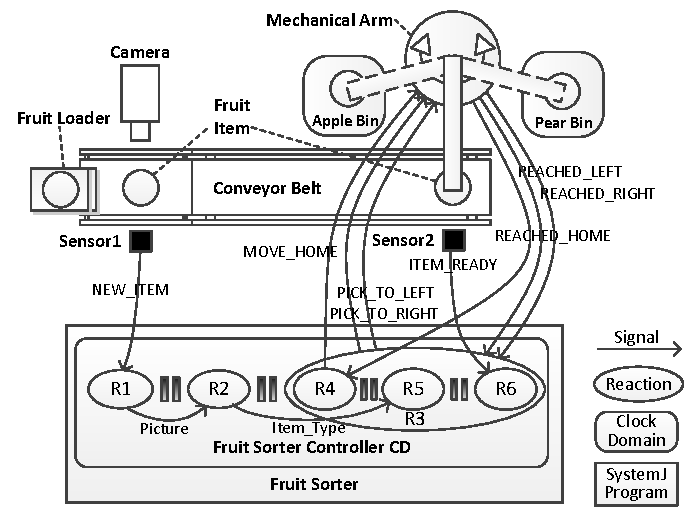
\includegraphics[scale=0.6]{fsorter}\label{fig:2a}}
  \qquad
  \subfloat[Fruit sorter controller clock-domain implementation in SystemJ]{
    \scalebox{0.7}{\usebox{\verbboxx}}
  \label{fig:4}}
  \caption{Fruit sorter control system}
  \label{fig:2}
\end{figure}

As shown in Figure~\ref{fig:2}, the fruit sorter consists of a fruit
loader, a conveyor belt, a mechanical arm, a camera and two sensors.
The fruit loader places fruit items on the left end of conveyor belt at
a constant speed and the conveyor belt moves from left to right carrying
fruit items. The structure of SystemJ program controlling the fruit
sorter controller is also shown in Figure~\ref{fig:2}. The program
contains only one synchronous clock-domain consisting of six reactions
(from R1 to R6). The presence of a fruit item loaded at the left end of
the conveyor belt is detected by Sensor 1 that produces an input signal
NEW\_ITEM to R1. Upon arrival of this signal, a picture of the fruit is
taken in R1 and analyzed to determine the type of the item (either apple
or pear in this example) in R2. This analysis is then used to sort the
fruit into the appropriate bin via a Mechanical sorting arm.

Reactions R4-R6 wait for three input signals in parallel before
performing actual sorting operation: (1) the Item\_Type signal from R2,
(2) ITEM\_READY signal produced by Sensor 2, indicating that a fruit
item is present at the right end of the conveyor belt and ready to be
sorted and (3) REACHED\_HOME signal indicating the mechanical arm has
completed the previous sorting procedure. Upon the arrival of all these
three input signals, R3 emits PICK\_TO\_LEFT or PICK\_TO\_RIGHT signal
to indicate to the mechanical arm to pick the item and move to the
correct bin, R3 then awaits for the REACHED\_LEFT or REACHED\_RIGHT
signal indicating that the mechanical arm has reached atop the correct
bin and dropped the item, then MOVE\_HOME signal is emitted to bring the
mechanical arm back to its initial position. 


% \begin{figure}[t!]
%   \centering
%   \caption{Fruit sorter controller clock-domain implementation in SystemJ}
%   \label{fig:4}
% \end{figure}

The SystemJ program implementing this control logic is shown in
Figure~\ref{fig:4}. There are two hard real-time requirements for the
control logic: (1) the time spent on item recognition should be shorter
than the incoming input signal NEW\_ITEM, else, the type of the fruit
cannot be recognized and (2) the mechanical arm should sort items faster
than the inter-arrival time of the input signal ITEM\_READY, else, the
fruit will not be placed into the bin and will drop off the conveyor
belt. These timing constraints essentially mean that the WCRT for
synchronous fruit sort controller should be shorter than the
inter-arrival time of input events.


\subsection{Static WCRT analysis of a SystemJ synchronous clock-domain}
\label{sec:static-wcrt-analysis}

In order to guarantee the aforementioned timing requirements we need to
statically determine the WCRT of the fruit sorter controller
clock-domain. The static analysis performed to estimate the WCRT of any
synchronous SystemJ clock-domain in described in~\cite{LiMS14}. Here in
we give a brief overview of the procedure.

\begin{lrbox}{\verbbox}
  \begin{minipage}[b]{0.5\linewidth}
    \begin{Verbatim}[numbers=left,commandchars=+\[\]]
public class FruitSorterController {
 //signal NEW_ITEM declaration
 private static Signal NEW_ITEM;
 ...//other signal and object declarations
 public static void init () {
  NEW_ITEM = new Signal();
 }
 public static void main(String args[]){
  init();
  while(true){
   //poll on the method call request from ReCOP
   int methodnum = Native.rd(Const.METHOD_NUM);
   switch(methodnum){
    case 0: ...
    ...
    //Call method representing action node
    //in AGRC
    case 24: Native.wr(RESULT_REG,
    MethodCall24_0());
   }
  }
 }
 private static boolean MethodCall24_0(){+label[fig:5bl1]
   // Compiled from Figure +ref[fig:4], line +ref[fig:4l1]
   imm_thread_4 = Camera.takepicture();
   //signal value emission
   picture_1.setValue(imm_thread_4);+label[fig:5bl2]
 }
}
    \end{Verbatim}
  \end{minipage}
\end{lrbox}

\begin{figure}[t!]
  \centering 

  \subfloat[The AGRC intermediate format for the fruit sorter controller
  clock-domain]{
    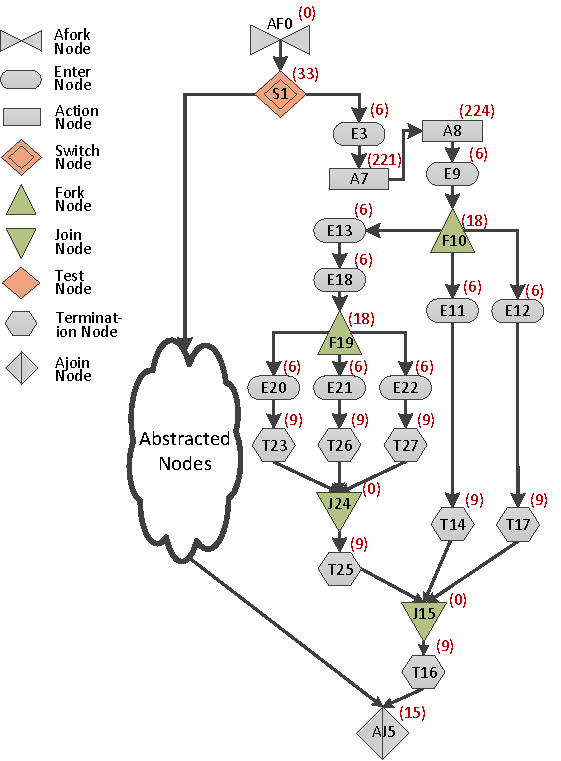
\includegraphics[scale=0.6]{agrc}
    \label{fig:5a}
  }
  \qquad
  \subfloat[The generated back-end Java code for JOP]{
    \scalebox{0.7}{\usebox{\verbbox}\label{fig:5b}}
  }
  \caption{AGRC intermediate format and generated back-end code for
    TP-JOP architecture}
  \label{fig:5}
\end{figure}

Every SystemJ clock-domain is compiled into an intermediate format
called the \textit{Asynchronous Graph Code} (AGRC)~\cite{amal10}. The
AGRC format of the fruit sorter controller clock-domain is shown in
Figure~\ref{fig:5a}. The AGRC intermediate format is akin to the
control-flow graph of a standard programming language, except that it
also encodes parallelism and state representation specific to SystemJ. A
single clock-domain transition from the start of a tick to the end of a
tick is a single traversal of the AGRC graph.

Every AGRC starts with the \texttt{AforkNode} representing forking of
multiple clock-domains, in case of the fruit sorter controller, a single
clock-domain is forked. The \texttt{Enter} and \texttt{Switch} nodes
together encode the state information. The \texttt{Enter} node sets the
value of a \texttt{Switch} node in any given program transition. The
\texttt{Switch} node then uses this value in the next tick to choose a
branch for execution. The synchronous parallelism is captured using
\texttt{Fork} and \texttt{Join} nodes. Every \texttt{Fork} node forks
multiple synchronous parallel reactions for execution, which are then
synchronized to the clock-domain tick at the \texttt{Join} node. The
signal emissions and Java data-computations are captured within the
\texttt{Action} nodes. The \texttt{Test} nodes are used for branching on
signal statuses. Finally, \texttt{Terminate} nodes, capture the
termination context of the currently executing tick. A program is
considered alive and ready to execute the next tick if the AGRC pass
terminates with value of 1, else a value of 0 means completion of the
program and all further program transitions are disabled.

The AGRC graph needs to be annotated with timing information in order to
compute the WCRT of the clock-domain. As stated previously, all
\textit{Control Nodes}, i.e., all nodes in the AGRC, except for
\texttt{Action} nodes encapsulating Java data-computations are executed
on the ReCOP and hence, their timing information can be easily computed,
as all native ReCOP instructions take 3 clock cycles to execute. The
\textit{Java Data Nodes} (JDN) are dispatched, encapsulated within
individual Java methods (see Figure~\ref{fig:5b}, line~\ref{fig:5bl1}),
for execution on JOP. One needs to compute the \textit{Worst Case
  Execution Time} (WCET) for each of these JDNs, using the JOP provided
worst case analysis tool~\cite{msch05}. The computed worst case
execution times for both: CNs and JDNs are back annotated onto the AGRC
shown by the numeric annotations on the AGRC nodes in
Figure~\ref{fig:5}. Once, annotated, the AGRC model is further
translated into a labeled transition system (LTS) for input into the
Uppaal model-checker~\cite{gbeh04}. A computational tree logic
(CTL)~\cite{clarke-book00} property of the form: \mbox{$A[] (wcrt <
  num)$}, which informally asks the model-checker to \textit{verify}
that there exists no path in the program with a wcrt value greater than
some number $num$. The integer value $wcrt$ is incremented on the LTS by
the WCET value of the AGRC node encountered.

This model-checking approach to computing the WCRT of a SystemJ
clock-domain is essential, because SystemJ clock-domains are
\textit{open} systems, unlike standard transformational programs and
hence, all possible paths need to be explored to guarantee find the
WCRT of a SystemJ clock-domain.

\section{A new memory model for SystemJ}
\label{sec:new-memory-model}

The WCRT approach described above is suitable \textit{only} for programs
that do not invoke \textit{Garbage Collection} (GC), since the GC
execution time is unaccounted for in the aforementioned WCRT
analysis. The main reason for this lack of GC incorporation is that GC
cycle time cannot be \textit{practically} bounded as the number of heap
allocations in a Java program depends upon the application and during
garbage collection a linked list of allocated objects needs to be
traversed as one of the collection phases.

One needs to include the GC time within the WCRT analysis of SystemJ
clock-domain for the WCRT analysis to be of any practical use. The very
first approach might be to include an incremental RTGC as described in
Section~\ref{sec:introduction}, but all current RTGC proposals require
preemptive scheduling, which does not bode well with the atomic tick
based execution of SystemJ clock-domains. Giving up on atomicity of
SystemJ clock-domain execution is not a viable option, since atomic tick
based clock-domain execution is the corner stone for formal verification
and WCRT analysis of synchronous programs. Of course, an RTGC might be
scheduled in the slack time -- time between completion of a clock-domain
transition and arrival of next set of input events, but one still
suffers from the problem of unbounded GC cycle time, since a GC cycle
needs to complete within the available slack.

Our solution to the above problem is to divide the heap space into two
parts: a bounded permanent heap and a transient heap with bump pointer
based object allocation and a simple pointer reset based garbage
collection, which are both bounded and efficient.

Signals (valued or pure) are the only communication primitive within a
SystemJ clock-domain. Upon emission of a valued signal, its status and
value become visible to the other reactions in the \textit{next}
clock-domain tick transition. Signals, internally themselves implemented
as Java objects (see Figure~\ref{fig:5b}), are alive throughout the
lifetime of the application. The new heap organization is based on one
\textbf{key insight}; there are two types of Java objects in a SystemJ
clock-domain:
\begin{enumerate}
\item \textit{Permanent objects}: Java objects that are emitted via
  signals. These objects like signals are potentially alive during the
  whole life time of the application.
\item \textit{Transient objects}: Java objects that are created
  internally for computation, but are never emitted via
  signals. Transient objects are only alive during a single clock-domain
  tick transition and can be garbage collected at the end of the
  transition.
\end{enumerate}

The basic idea is to allocate the permanent objects, we consider signals
to be permanent objects as well, within a special memory area called
\textit{permanent heap} and allocate all transient objects within a
\textit{transient heap}. The transient heap gets garbage collected at
the end of every clock-domain tick transition, by simply resetting the
allocation pointer to the start of the transient heap space. With this
change, the runtime Java memory organization for JOP is compared with
the original GC based memory organization in Figure~\ref{fig:6}.

\begin{figure}[t!]
  \centering
  \subfloat[Original JOP runtime memory organization]{
    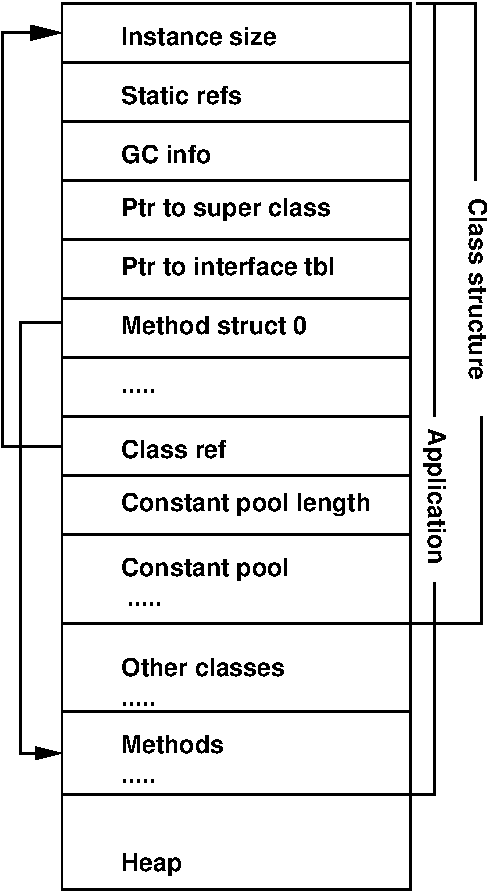
\includegraphics[scale=0.4]{jvmmem}\label{fig:6a}
  }
  \qquad
  \subfloat[New JOP runtime memory organization]{
    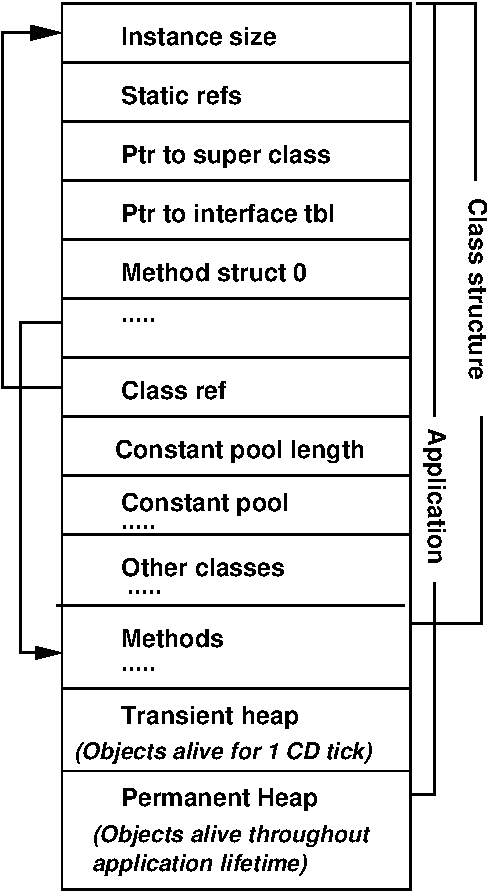
\includegraphics[scale=0.4]{jvmmemn}\label{fig:6b}
  }
  \qquad
  \subfloat[The tool-chain flow]{
    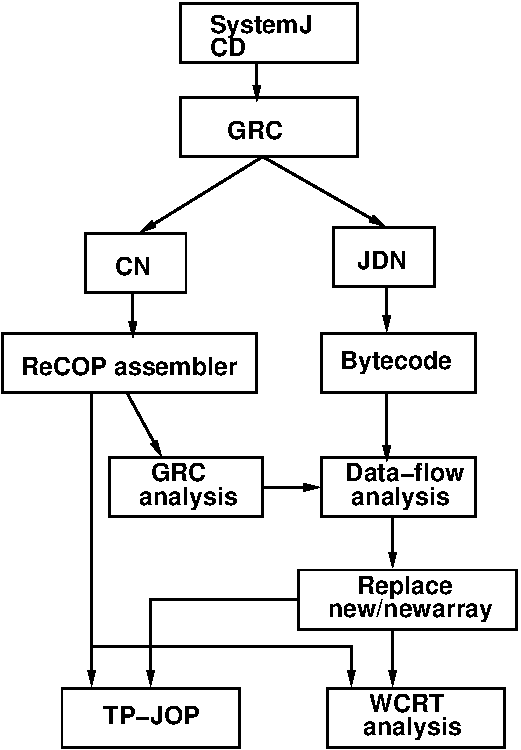
\includegraphics[scale=0.4]{tcflow}
    \label{fig:6c}
  }
  \caption{The tool-chain flow along with the Java runtime memory
    structure in JOP, before and after transformation. The Java stack is
    on separate physical memory as shown in Figure~\ref{fig:3}.}
  \label{fig:6}
\end{figure}

Both runtime memory organizations; original (Figure~\ref{fig:6a}) and
new (Figure~\ref{fig:6b}) consists of a number of common elements
required to execute every Java application such as, the constant pool,
method structure table for instance method invocation, references to
static objects, etc. The major point of difference is that the
\textit{GC info} word does not exist in the new runtime memory structure
and the \textit{heap} space is divided into two parts; the transient
heap and the permanent heap. Looking at the runtime memory organization
two aspects become very important:

\begin{itemize}
\item There should be no pointer pointing from the permanent heap to the
  transient heap, else an application might terminate at runtime with a
  \texttt{NullPointer} exception. Or in the much worse scenario, an
  incorrect value might be read, in which case the application will
  be functionally incorrect!
\item The permanent heap is never garbage collected and hence, permanent
  heap space should be judiciously allocated. In fact, we need to bound
  the permanent heap space at compile time.
\end{itemize}

In the rest of the paper we describe compiler transformations that
achieve the described memory reorganization.


\section{Compiler analysis for static memory allocations}
\label{sec:comp-analys-stat}

The complete compiler tool-chain flow in shown in
Figure~\ref{fig:6c}. The SystemJ program is first compiled into the
intermediate AGRC format. Next, the control nodes (CN) and the Java data
nodes (JDN) are split and compiled separately into ReCOP native assembly
and Java bytecode, respectively, for execution on the TP-JOP
platform. Two types of compiler analysis are then performed on the
produced native ReCOP assembler and Java bytecode, respectively: (1)
AGRC analysis is used to determine the \textit{must} and \textit{may}
Java reachable methods from any given Java program point and (2)
\textit{forward} and \textit{backward} data-flow analysis to find the
objects/arrays that need to be allocated to the permanent heap.

\begin{lrbox}{\eone}
  \begin{minipage}[b]{0.5\linewidth}
    \begin{Verbatim}[numbers=left,commandchars=\\\[\]]
int signal S;\label[l1]
int a = 0;\label[l2]
a = a + 1;\label[l3]
pause;\label[l7]
emit S(a);\label[l4]
a = a + 1;\label[l5]
emit S(a);\label[l6]
    \end{Verbatim}
  \end{minipage}
\end{lrbox}
\begin{lrbox}{\etwo}
  \begin{minipage}[b]{0.7\linewidth}
    \begin{Verbatim}[numbers=left,commandchars=\\\[\]]
public class FruitSorterController {
 //signal S declaration
 private static Signal S;
 private static int a;
 public static void init () {
  S = new Signal();
 }
 public static void main(String args[]){
  init();
  while(true){
   //poll on the method call request from ReCOP
   int methodnum = Native.rd(Const.METHOD_NUM);
   switch(methodnum){
    case 0: ...
    ...
    //Call method for 
    //lines \ref[l2] - \ref[l4] (Figure~\ref[fig:7a])
    case 1: Native.wr(RESULT_REG,
    MethodCall1_0());
    //Call method for 
    //lines \ref[l5] - \ref[l6] (Figure \ref[fig:7a])
    case 2: Native.wr(RESULT_REG,
    MethodCall2_0());
   }
  }
 }
 private static boolean MethodCall1_0(){
   a = 0;//line \ref[l2], Figure \ref[fig:7a]
   a = a + 1;//line \ref[l3], Figure \ref[fig:7a]
   S.setValue(new Integer(a));
 }
 private static boolean MethodCall2_0(){
   a = a + 1;
   S.setValue(new Integer(a));
 }
}
    \end{Verbatim}
  \end{minipage}
\end{lrbox}

\begin{figure}[t!]
  % \centering
  \subfloat[SystemJ code snippet]{
    \scalebox{0.7}{\usebox{\eone}}
    \label{fig:7a}
  }
  \qquad
  \subfloat[Produced Java code]{
    \scalebox{0.7}{\usebox{\etwo}}
    \label{fig:7b}
  }
  \caption{Example showing the need for AGRC and data-flow analysis of a SystemJ program}
  \label{fig:7}
\end{figure}

The need for these two types of analysis can be explained using the
simple example in Figure~\ref{fig:7a}. The SystemJ code snippet declares
a valued signal \texttt{S}, and an integer variable \texttt{a}. This
variable is incremented and emitted via signal \texttt{S}. After
emission the variable is incremented again. For this SystemJ program,
two methods are produced in the back-end Java code for execution on
JOP. The first method \texttt{MethodCall1\_0} initializes the
\texttt{a}, increments it and then sets the value of the signal
\texttt{S} as the object \texttt{a}. The second method call
\texttt{MethodCall2\_0} increments the variable \texttt{a} and changes
the object reference of signal \texttt{S}.

Our objective is to find out all the \textit{program-points} that
allocate a new object, whose returned reference is set as a signal value
(via the \texttt{setValue} virtual method call on the signal object). We
perform data-flow analysis (ReachDef analysis~\cite{steven1997advanced}
to be exact) to find out such program points in the Java program
generated for execution on JOP (e.g., Figure~\ref{fig:7b}). Fields or
method local object references might be set as signal values and hence,
our data-flow analysis is a context and flow-sensitive intra-procedural
and inter-procedural analysis, i.e., the data-flow analysis not only
examines a Java method, but also needs to traverse the call-graph of the
generated Java program.

A call-graph generated from \textit{just} the Java program is
incomplete, since method calls that \textit{must happen before} a given
program point \textit{appear} as \textit{may happen before} a given
program point. Consider the SystemJ program in Figure~\ref{fig:7a}, we
know for sure that program point at line~\ref{l3} \textit{must} be
executed before program point at line~\ref{l5}. But, in the generated
Java program (Figure~\ref{fig:7b}), the sequential control-flow of the
\textit{SystemJ program} has been turned into a branching
control-flow. Just looking at the Java program one can only state with
certainty that method \texttt{MethodCall1\_0} \textit{may} be called
before method \texttt{MethodCall2\_0}. More disconcertingly, just
looking at the Java program, one can even say that method
\texttt{MethodCall2\_0} may be called before \texttt{MethodCall1\_0},
since the dependence edge clear in the SystemJ program is lost in the
generated Java program. The AGRC analysis step produces the may and must
method callers for any callee in the generated Java code. Note that we
cannot produce a single Java method call coalescing the two Java
methods: \texttt{MethodCall1\_0} and \texttt{MethodCall2\_0}, because
there is a control node \texttt{pause} that needs to be executed on
ReCOP. We describe these AGRC and the data-flow analysis steps in the
next sections.

\subsection{AGRC analysis}
\label{sec:agrc-analysis}

Give formal definition of may and must. Then describe the algorithm that
given a method, the callee method, gives the may and must caller
methods.

\subsection{Data-flow analysis}
\label{sec:data-flow-analysis}

\begin{figure}[t!]
  \centering
  \subfloat[Points-to from permanent heap to transient heap]{
    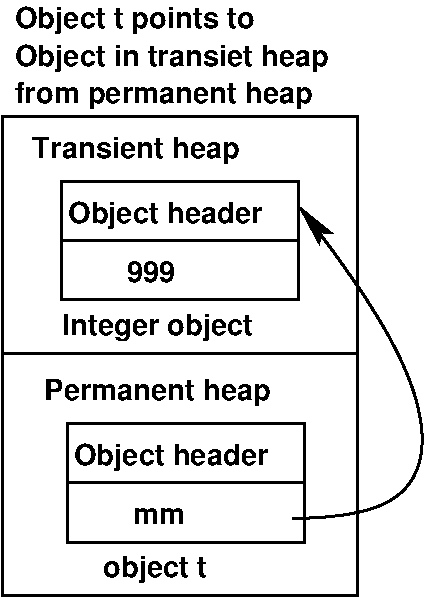
\includegraphics[scale=0.45]{ptp1}
    \label{fig:9a}
  }
  \qquad
  \subfloat[Points-to only in permanent heap]{
    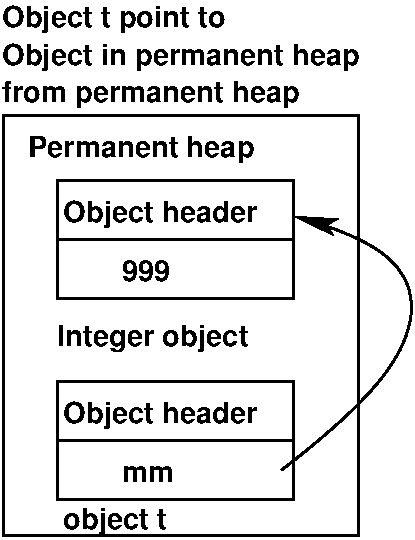
\includegraphics[scale=0.45]{ptp2}
    \label{fig:9b}
  }
  \caption{The points-to problem}
  \label{fig:9}
\end{figure}

As stated previously, we have an intra and inter-procedural
flow-sensitive data-flow analysis to locate the program points that
allocate new objects (or arrays) whose returned references are set as
signal values. Java bytecode is not an ideal format for performing such
data-flow analysis~\cite{vallee1999soot,hubert2011sawja}, because the
stack interacts with each bytecode operation, this means that data-flow
analysis would need simulating the stack state. In order to avoid
simulating the stack itself, we (like other Java static analysis
frameworks~\cite{vallee1999soot,hubert2011sawja}) first convert the
bytecode into a register-transfer level (RTL) intermediate format. For
this work, we have used the OCaml~\cite{leroy1998ocaml} based Java
static analysis framework; Sawja's~\cite{hubert2011sawja} intermediate
RTL format called \textit{Bytecode Intermediate Representation} (BIR).

\newsavebox{\exinv}
\begin{lrbox}{\exinv}
  \begin{minipage}[b]{0.7\linewidth}
    \begin{Verbatim}[numbers=left,commandchars=\\\[\]]
private static Signal S;
public static void main(String args[]){
 Integer A = 0;\label[exinv:l1]
 Integer B = 1;\label[exinv:l2]
 S.setValue(A);\label[exinv:l3]
}
    \end{Verbatim}
  \end{minipage}
\end{lrbox}

\newsavebox{\exinvt}
\begin{lrbox}{\exinvt}
  \begin{minipage}[b]{0.7\linewidth}
    \begin{Verbatim}[numbers=left,commandchars=\\\[\]]
iconst_0 \label[exinvt:l0]
invokestatic  #2// valueOf:(I)Ljava/lang/Integer;\label[exinvt:l1]
astore_1 \label[exinvt:l2]     
iconst_1 \label[exinvt:l3]
invokestatic  #2// valueOf:(I)Ljava/lang/Integer;\label[exinvt:l4]
astore_2\label[exinvt:l5]
return        
    \end{Verbatim}
  \end{minipage}
\end{lrbox}

\newsavebox{\exinvtt}
\begin{lrbox}{\exinvtt}
  \begin{minipage}[b]{0.7\linewidth}
    \begin{Verbatim}[numbers=left,commandchars=\\\[\]]
new #3 // class java/lang/Integer\label[exinvtt:l1]
dup
iload_0
invokespecial #10 // Method "<init>":(I)V
areturn
    \end{Verbatim}
  \end{minipage}
\end{lrbox}
\begin{figure}[t!]
  \centering
  \subfloat[Example Java code snippet]{
    \scalebox{0.6}{\usebox{\exinv}}
    \label{fig:10a}
  }
  \qquad
  \subfloat[Produced Java bytecode]{
    \scalebox{0.6}{\usebox{\exinvt}}
    \label{fig:10b}
  }
  \qquad
  \subfloat[The bytecode for method \texttt{valueOf} in Integer class]{
    \scalebox{0.6}{\usebox{\exinvtt}}
    \label{fig:10c}
  }
  \caption{Inadvertent object sharing problem}
  \label{fig:10}
\end{figure}
\newsavebox{\algone}
\begin{lrbox}{\algone}
  \begin{minipage}[b]{0.5\linewidth}
    \begin{algo}
      \SetKwData{Let}{let}
      \SetKwFunction{Steptwo}{Step2}
      \SetKwFunction{Reachable}{ReachableMethods}
      \SetKwFunction{Size}{sizeof}
      \KwIn{program: Program in RTL format} 
      \BlankLine
      \tcc*[h]{$pp$ is the multi-set of program points}\\
      \Let \textbf{global} $pp \leftarrow \emptyset$\;\label{algone:l1}
      \Let $M \leftarrow$ \texttt{main}\;
      \Let $M \leftarrow$ \Reachable(\texttt{main}) $\cup$ $\{M\}$\;
      \Let $size \leftarrow$ \Size(signal class)\;
      \ForEach{$m \in M$} {
        \Let pp $\leftarrow$ ($size$, get in $m$, program points initializing signals)\;
      }
      \Steptwo(program,pp,\texttt{main})\;
    \end{algo}
  \end{minipage}
\end{lrbox}

\newsavebox{\algtwo}
\begin{lrbox}{\algtwo}
  \begin{minipage}[b]{0.5\linewidth}
    \begin{algo}
      \SetKwData{Let}{let}
      \SetKwFunction{Code}{code}
      \SetKwFunction{Signalset}{signalSet}
      \SetKwFunction{Emits}{emits}
      \SetKwFunction{InvokesMethod}{invokesMethod}
      \SetKwFunction{Steptwo}{Step2}
      \SetKwFunction{GetMethod}{getInvoked}
      \SetKwFunction{Stepthree}{Step3}
      \KwIn{program: Program in RTL format} 
      \KwIn{pp: Set of program points} 
      \KwIn{\texttt{method}: Method to scan for signal emissions} 
      \BlankLine
      \Let $S \leftarrow$ \Signalset(pp)\;
      \Let $C \leftarrow$ \Code(\texttt{method})\;
      \Let $PPC \leftarrow \emptyset$\;
      \ForEach{$c \in C$}{\label{algtwo:l1}
        \If{\Emits($c$,$S$)}{
          $PPC \leftarrow PPC\ \cup \{c\}$\;
        }
      }\label{algtwo:l2}
      \Stepthree(program,$PPC$,$C$)\;
      \ForEach{$c \in C$}{
        \If{\InvokesMethod($c$)}{
          \Steptwo(program,$c$,\GetMethod($c$))\;
        }
      }
    \end{algo}
  \end{minipage}
\end{lrbox}

\newsavebox{\algthree}
\begin{lrbox}{\algthree}
  \begin{minipage}[b]{0.5\linewidth}
    \begin{algo}
      \SetKwData{Let}{let}
      \SetKwFunction{Code}{code}
      \SetKwFunction{Signalset}{signalSet}
      \SetKwFunction{Emits}{emits}
      \SetKwFunction{GetExpr}{getExpr}
      \SetKwFunction{AffectsFields}{affectsFields}
      \SetKwFunction{AffectsVars}{affectsVars}
      \SetKwFunction{StepFour}{Step4}
      \SetKwFunction{StepFive}{Step5}
      \KwIn{program: Program in RTL format} 
      % \KwIn{pp: Set of program points} 
      \KwIn{$PPC$: Set of program points affected} 
      \KwIn{$C$: code of the method containing $PPC$}
      \BlankLine
      \ForEach{$ppc \in PPC$}{
        \uIf{\AffectsFields(\GetExpr($ppc$))}{
          \Let $pp \leftarrow pp\ \cup$ \StepFour(program,$ppc$,\GetExpr($ppc$),$C$)\;
        }
        \uElseIf{\AffectsVars(\GetExpr($ppc$))}{
          \Let $pp \leftarrow pp\ \cup$ \{\StepFive(program,$ppc$,\GetExpr($ppc$),$C$)\}\;
        }
        \lElse{\texttt{raise error}}
      }
    \end{algo}
  \end{minipage}
\end{lrbox}

\newsavebox{\algfour}
\begin{lrbox}{\algfour}
  \begin{minipage}[b]{0.5\linewidth}
    \begin{algo}
      \SetKwData{Let}{let}
      \SetKwFunction{Code}{code}
      \SetKwFunction{GetFields}{getFields}
      \SetKwFunction{Escape}{escape}
      \SetKwFunction{StepSix}{Step6}
      \SetKwFunction{FieldOf}{fieldOf}
      \SetKwFunction{HasRefFields}{hasRefFields}
      \SetKwFunction{GetAffectedFeilds}{getAffectedFields}
      \SetKwFunction{StepThree}{Step3}
      \SetKwFunction{Max}{max}
      \SetKwFunction{SizeOf}{sizeof}
      \KwIn{program: Program in RTL format} 
      \KwIn{$ppc$: Affected program point} 
      \KwIn{$pexpr$: Expression affecting field} 
      \KwIn{$C$: code of the method containing $ppc$} 
      \BlankLine
      \Let $f \leftarrow$ \FieldOf($pexr$)\;
      \Let ($size$,$defs$) $\leftarrow$ \StepSix(program,$ppc$,$f$,$C$)\;
      \lIf {$size \neq 0$} {\Return ($size$,$defs$)}\;
      \ForEach {$d \in defs$} { \label{step4:s}
        \uIf{!\Escape(program,$C$,$d$)} {
          \If {\HasRefFields($f$)} {
            % start2
            \Let $PPC \leftarrow$ \GetAffectedFeilds(\GetFields($f$))\;
            \StepThree(program,$PPC$,$C$)\;
          }
        }
        \lElse {
          \texttt{raise error}\;
        }
      }
      \Let $size \leftarrow$ \Max(\SizeOf($defs$))\; \label{step4:e}
      \Return ($size$,$defs$)\;
    \end{algo}
  \end{minipage}
\end{lrbox}

\newsavebox{\algfive}
\begin{lrbox}{\algfive}
  \begin{minipage}[b]{0.5\linewidth}
    \begin{algo}
      \SetKwData{Let}{let}
      \SetKwFunction{Code}{code}
      \SetKwFunction{GetFields}{getFields}
      \SetKwFunction{Escape}{escape}
      \SetKwFunction{StepSeven}{Step7}
      \SetKwFunction{VarOf}{varOf}
      \SetKwFunction{HasRefFields}{hasRefFields}
      \SetKwFunction{GetAffectedFields}{getAffectedFields}
      \SetKwFunction{StepThree}{Step3}
      \SetKwFunction{Max}{max}
      \SetKwFunction{SizeOf}{sizeof}
      \KwIn{program: Program in RTL format} 
      \KwIn{$ppc$: Affected program point} 
      \KwIn{$pexpr$: Expression affecting field} 
      \KwIn{$C$: code of the method containing $ppc$} 
      \BlankLine
      \Let $v \leftarrow$ \VarOf($pexr$)\;
      \Let $defs \leftarrow$ \StepSeven(program,$ppc$,$v$,$C$)\;
      \ForEach {$d \in defs$} {
        \uIf{!\Escape(program,$C$,$d$)} {
          \If {\HasRefFields($v$)} {\label{algfive:l1}
            % start2
            \Let $PPC \leftarrow$ \GetAffectedFields(\GetFields($v$))\;
            \StepThree(program,$PPC$,$C$)\;
          }\label{algfive:l2}
        }
        \lElse {
          \texttt{raise error}\;
        }
      }
      \Let $size \leftarrow$ \Max(\SizeOf($defs$))\;
      \Return ($size$,$defs$)\;
    \end{algo}
  \end{minipage}
\end{lrbox}

\newsavebox{\algsix}
\begin{lrbox}{\algsix}
  \begin{minipage}[b]{0.5\linewidth}
    \begin{algo}
      \SetKwData{Let}{let}
      \SetKwFunction{Escape}{escape}
      \SetKwFunction{ReachDef}{reachDef}
      \SetKwFunction{GetAllFields}{getAllFields}
      \SetKwFunction{GetCallers}{getCallers}
      \SetKwFunction{GetCallerPPC}{getCallerPPC}
      \SetKwFunction{GetVarSetting}{getVarSetting}
      \SetKwFunction{StepSeven}{Step7}
      \KwIn{program: Program in RTL format} 
      \KwIn{$ppc$: Affected program point} 
      \KwIn{$f$: Field affected} 
      \KwIn{$C$: code of the method containing $ppc$} 
      \BlankLine
      \Let $ofields \leftarrow$ \GetAllFields($C$) $\backslash$ \{$f$\} \;\label{algsix:l1}
      \Let $pcs \leftarrow$ \ReachDef($ppc$,$f$)\;
      \uIf {$pcs \neq \emptyset$} {
        \Let $defs \leftarrow \emptyset$\;
        \ForEach {$pc \in pcs$} {
          \Let $vf \leftarrow$ \GetVarSetting($f$,$pc$)\;
          \Let $tt \leftarrow$ \StepSeven(program,$pc$,$vf$,$C$)\;\label{algsix:s7c}
          \uIf {all other $field \in ofields$ have same $tt$} {
            \tcc*[h]{Concat in set $defs$}\\
            $defs \leftarrow defs\ \cup tt$\;
          }\lElse {
            \tcc*[h]{Append a new set in $defs$}\\
            $defs \leftarrow defs\ \cup \{tt\}$\;
          }
        }
        \Return (0,$defs$)\;
      }\label{algsix:l2}
      \Else {\label{algsix:l3}
        \tcc*[h]{Inter-procedural analysis}\\
        \tcc*[h]{Get all callers, including from AGRC analysis}\\
        \Let $Callers \leftarrow$ \GetCallers($C$)\;
        \lIf {$Callers = \emptyset$} \texttt{raise Not\_init $f$}\;
        \ForEach {$caller \in Callers$} {
          \Let $defs \leftarrow$ \StepSix(program,\GetCallerPPC($C$),$f$,$caller$)\;
          \tcc*[h]{Same as Figure~\ref{fig:8d} lines~\ref{step4:s}-\ref{step4:e}}
          \Return ($size$,$defs$)\;
        }
      }\label{algsix:l4}
    \end{algo}
  \end{minipage}
\end{lrbox}

\begin{figure}[h!]
  \centering
  \subfloat[Step1:Scan signal initialization]{
    \scalebox{0.7}{\usebox{\algone}}
    \label{fig:8a}
  }
  \qquad
  \subfloat[Step2: Scan \texttt{setValue} method calls]{
    \scalebox{0.7}{\usebox{\algtwo}}
    \label{fig:8b}
  }
  \qquad
  \subfloat[Step3: For every affected field/variable get the object
  initialization program points]{
    \scalebox{0.7}{\usebox{\algthree}}
    \label{fig:8c}
  }
  \qquad
  \subfloat[Step4: Get object initialization for affected field]{
    \scalebox{0.7}{\usebox{\algfour}}
    \label{fig:8d}
  }

  \subfloat[Step5: Get object initialization for affected variables]{
    \scalebox{0.7}{\usebox{\algfive}}
    \label{fig:8e}
  }
  \qquad
  \subfloat[Step6: Search object initialization for affected field]{
    \scalebox{0.7}{\usebox{\algsix}}
    \label{fig:8f}
  }

  \caption{Data-flow analysis algorithm}
  \label{fig:8}
\end{figure}

\newsavebox{\algseven}
\begin{lrbox}{\algseven}
  \begin{minipage}[b]{0.5\linewidth}
    \begin{algo}
      \SetKwData{Let}{let}
      \SetKwFunction{Escape}{escape}
      \SetKwFunction{ReachDef}{reachDef}
      \SetKwFunction{NotReachable}{notReachable}
      \SetKwFunction{GetAllFields}{getAllFields}
      \SetKwFunction{GetExpr}{getExpr}
      \SetKwFunction{VarOf}{varOf}
      \SetKwFunction{GetVarSetting}{getVarSetting}
      \SetKwFunction{StepFour}{Step4}
      \KwIn{program: Program in RTL format} 
      \KwIn{$ppc$: Affected program point} 
      \KwIn{$v$: Variable affected} 
      \KwIn{$C$: code of the method containing $ppc$} 
      \BlankLine
      \Let $pcs \leftarrow$ \ReachDef($ppc$,$v$)\;\label{algseven:l1}
      \lIf{$pcs = \emptyset$} {\texttt{raise Not\_init}}\;\label{algseven:l3}
      \Let $defs \leftarrow \emptyset$\;
      \ForEach {$pc \in pcs$} {
        \uIf {\GetExpr($pc$) is \texttt{New} \textbf{or} \GetExpr($pc$) is \texttt{NewArray}} {
          $defs \leftarrow defs\ \cup \{pc\}$\;\label{algseven:l2} 
        }
        \uElseIf {\GetExpr($pc$) is \texttt{AffectField}} {
          \Let $expr \leftarrow$ \GetExpr($pc$)\;
          \Let (\_,$defs$) $\leftarrow$ \StepFour(program,$pc$,$expr$,$C$)\;
        }
        \uElseIf {\GetExpr($pc$) is \texttt{AffectVar}}{
          \Let $v \leftarrow$ \VarOf(\GetExpr($pc$))\;
          \Let (\_,$defs$) $\leftarrow$ \StepSeven(program,$pc$,$v$,$C$)\;
        }
        \Else {\label{algseven:l4}
          \tcc*[h]{Cannot handle new outside current method allocation}\\
          \texttt{raise Not\_handled}
        }\label{algseven:l5}
      }
      \tcc*[h]{Make sure that definitions are not reachable from each other}\\
      \If {$|defs| > 1$} {
        \textbf{assert}(\NotReachable($defs$))\;
      }
      \Return($defs$)\;
    \end{algo}
  \end{minipage}
\end{lrbox}

\newsavebox{\exone}
\begin{lrbox}{\exone}
  \begin{minipage}[b]{0.7\linewidth}
    \begin{Verbatim}[numbers=left,commandchars=\\\[\]]
private static Signal S;
private static boolean a_thread_2;
public static void init () {
 S = new Signal();\label[exone:siginit]
}
public boolean MethodCall0_4() {
 /* B and C should share the heap 
    and should be the max of the two sizes */
 b B = new b(33);
 c C = new c(1001,101);
 a t;
 /* Use polymorphism for equality */
 a_thread_2 = true;
 if (a_thread_2){
  int b1 = B.getb1();
  t = new b(b1);/*Making deep copies*/\label[exone:l1]
  ((b)t).bbb = new Integer(99);
 }
 else {
  int c1 = C.getc1();
  int c2 = C.getc2();
  t = new c(c1,c2);/*Making deep copies*/\label[exone:l2]
  ((c)t).mm = new Integer(999);\label[exone:l3]
 }
 /* Emit t via S */
 S.setValue(t);\label[exone:s2l1]
 if (a_thread_2)\label[exone:l3]
  /* Print */
  System.out.println(((b)S.getValue()).bb);
 else {
  /* Print */
  System.out.println(((c)S.getValue()).cc);
  System.out.println(((c)S.getValue()).ccc);
 }\label[exone:l4]
 return true;  
}
    \end{Verbatim}
  \end{minipage}
\end{lrbox}

\newsavebox{\extwo}
\begin{lrbox}{\extwo}
  \begin{minipage}[b]{0.7\linewidth}
    \begin{Verbatim}[numbers=left,commandchars=\\\[\]]
private static Signal S;
private static a A;
public static void main(String args[]){
 A = new a();\label[extwo:l2]
 A.b = new Integer (70);\label[extwo:l3]
 MethodCall0_0();
}
public boolean MethodCall0_0(){
 /* Test 1 */
 S.setValue(A);\label[extwo:l1]
 return false;
}
    \end{Verbatim}
  \end{minipage}
\end{lrbox}
\begin{figure}[t!]
  \ContinuedFloat
  \centering
  \subfloat[Step7: Search object initialization point for method local affected
  variable]{
    \scalebox{0.7}{\usebox{\algseven}}
    \label{fig:8g}
  }
  \qquad
  \subfloat[Example 1: variables and intra-procedural analysis]{
    \scalebox{0.7}{\usebox{\exone}}
    \label{fig:8h}
  }
  
  \subfloat[UML class hierarchy for classes \texttt{A}, \texttt{B} and
  \texttt{C} used in Figure~\ref{fig:8h} and~\ref{fig:8j}]{
    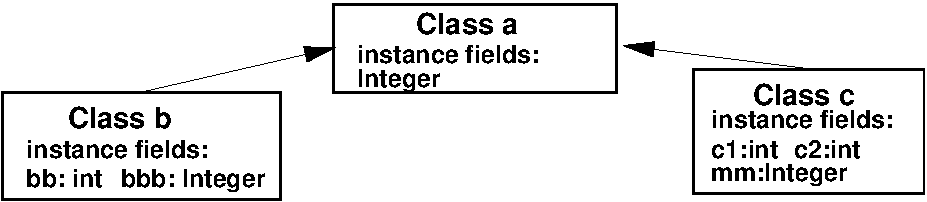
\includegraphics[scale=0.5]{umlex1}
    \label{fig:8i}
  }
  \qquad
  \subfloat[Example 2: Fields and inter-procedural analysis]{
    \scalebox{0.7}{\usebox{\extwo}}
    \label{fig:8j}
  }
  \caption{Data-flow analysis algorithm and related examples}
  \label{fig:8}
\end{figure}

Given the class file(s) in the RTL format, the data-flow analysis
carried out is shown in Figure~\ref{fig:8}. Being a relatively complex
procedure we use simple code examples to describe the data-flow analysis
procedure.

Consider the Java program in Figure~\ref{fig:8h}. This program consists
of a single signal \texttt{S}. Signal \texttt{S} is initialized in the
\texttt{init} method, next method \texttt{MethodCall0\_4} is called,
which initializes objects \texttt{B} and \texttt{C}, whose types
\texttt{b} and \texttt{c} are inherited from a single parent class
\texttt{a} as shown in Figure~\ref{fig:8i}. Object \texttt{t} of type
\texttt{a} is initialized to either type \texttt{b} or \texttt{c}
(line~\ref{exone:l1}, line~\ref{exone:l2}) if the Boolean
\texttt{a\_thread\_2} is \texttt{true} or not. Finally, \texttt{t} is
emitted via signal \texttt{S} and this emitted signal value is printed
again within a conditional branching construct
(lines~\ref{exone:l3}-\ref{exone:l4}).

\begin{compactitem}[$\bigstar$]
\item Step1 of the data-flow analysis algorithm (Figure~\ref{fig:8a})
  starts by scanning the Java program for program points initializing
  signals (e.g., method \texttt{init} in Figure~\ref{fig:8h}). A
  globally accessible multi-set $pp$ (Figure~\ref{fig:8a},
  line~\ref{algone:l1}) is defined that will hold all the program points
  initializing the objects that will be placed in the permanent
  heap. Step1 scans all reachable methods from the starting program
  point (usually the \texttt{main} method) for signal initialization and
  places these program points into the multi-set $pp$. Each individual
  set within the multi-set $pp$ consists of a one or more program points
  that initialize objects. After the scan phase, the set $pp$ holds
  $\{\{\mathtt{(5,init:\ref{exone:siginit}})\}\}$ for the example in
  Figure~\ref{fig:8h}. The first element of the tuple gives the
  \textit{instance} size of the \texttt{Signal} class, the second
  element is the initialization program point~\footnote{The
    initialization program point is actually at the bytecode level, but
    in this paper we keep the initialization points at the Java source
    code level for ease of understanding.} for the example in
  Figure~\ref{fig:8h}. If more than one signal is initialized, all these
  initializations are placed in separate sets within the multi-set
  $pp$. The reason for having a set rather than a multi-set for $pp$
  will become clear as we proceed with the example. Finally, Step2 is
  called to find all reachable program points from signal emissions that
  will be used for identifying objects that need to be placed in the
  permanent heap.
  
\item Step2 is a recursive procedure that scans all reachable methods
  for the \texttt{setValue} virtual method call on the signal objects
  (Figure~\ref{fig:8b}, lines~\ref{algtwo:l1}-\ref{algtwo:l2}). These
  program points are placed in the set $PPC$ for each reachable method
  individually. For the example in Figure~\ref{fig:8h}, the means
  scanning method \texttt{MethodCall0\_4} and placing the program point
  line~\ref{exone:s2l1} in set $PPC$. Finally, Step3 of the algorithm is
  called.
  
\item Step3 analyzes the emission expression for every program point in
  set $PPC$. A emitting expression can \textit{only} ever emit a method
  local variable (as in the case of Figure~\ref{fig:8h}) or a field (as
  in the case of our soon to come example in Figure~\ref{fig:8j}). For
  our current example, a variable is being emitted (or affected) and
  hence, Step5 is called.
  
\item Step5 analyzes the variable from the expression and calls Step7
  for analysis. Step7 is the main part of the algorithm that performs
  the reachability analysis to identify the program points initializing
  the objects to be placed in permanent heap. Before proceeding to
  Step7, let us assume that we have already obtained the correct program
  points from Step7 in set $defs$. For our current example, given that
  the emitting program point is~\ref{exone:s2l1},
  $defs = \{\ref{exone:l1},\ref{exone:l2}\}$. Looking at
  Figure~\ref{fig:8h}, it is clear that \texttt{t} can be initialized at
  either~\ref{exone:l1} or~\ref{exone:l2}, depending upon the value of
  variable \texttt{a\_thread\_2} during program execution. For each of
  these program points, Step5 guarantees that the object instance
  (equally the reference) does not \textit{escape} the
  method~\cite{choi1999escape}.~\footnote{Let $O$ be an object instance
    and $M$ be a method invocation. $O$ is said to escape $M$, if the
    lifetime of $O$ may exceed the lifetime of $M$.} If the object
  instance does not escape the method lifetime, then the algorithm
  checks if their are any reference fields, if so, Step3 is invoked for
  migrating these object allocations initializing these reference fields
  into permanent heap. Consider, the program point~\ref{exone:l2},
  object \texttt{t} is initialized as class \texttt{c} (for program
  point~\ref{exone:l1}, \texttt{t} is initialized and analyzed as class
  \texttt{b}), which has three fields: two (\texttt{c1} and \texttt{c2})
  are primitive fields, but the third: \texttt{mm} is a reference field
  (of type \texttt{Integer}). The \texttt{mm} reference field is
  initialized to an \texttt{Integer} object at program
  point~\ref{exone:l3}. Figure~\ref{fig:9a} shows the reference held by
  \texttt{mm} if Step3 is not carried out. Field \texttt{mm} points to
  an object in transient heap space, which violates the second
  requirement in Section~\ref{sec:new-memory-model}. Calling Step3,
  guarantees that all potential \textit{pointed-to} objects from the
  permanent heap are also migrated to the permanent-heap. Note that
  Step3 and Step5 are mutually recursive and hence perform a chained
  permanent heap migration as shown in Figure~\ref{fig:9b}.
  
  The final computation that Step5 performs is computing the size, which
  will be reserved in the permanent heap, of object \texttt{t}, given
  that $defs$ may have multiple (two in our current example)
  elements. The primary idea is to reserve maximum size amongst all
  different types being initialized. For the running example,
  \texttt{t}, can be of type \texttt{b} or \texttt{c} at program
  execution time. We compute the \textit{instance} size of both these
  types, 3 and 4, respectively~\footnote{By Java semantics, all fields
    of a parent class are inherited by the children classes and hence,
    the sizes for \texttt{b} and \texttt{c} is 3 and 4 words.} and
  reserve 4 words (plus object header) in permanent heap space. Step7
  returns multiple program points in set $defs$ \textrm{iff} these
  program points are mutually unreachable. This, guarantees that the
  reserved permanent heap space can be reused at runtime by both:
  program points in $defs$.
  \newline
  \begin{compactitem}[$\boxplus$]
  \item \textbf{Design decision}: We have consciously decided to not
    allow method local object instances from escaping because, it leads
    to trade-off between space utilization and functional
    correctness. If we allow, for example \texttt{t} in
    Figure~\ref{fig:8h}, to escape method \texttt{MethodCall0\_4}, then
    any of the reference fields of \texttt{t} (e.g., \texttt{mm}) might
    be reinitialized at some other program point. This program point
    would also then need to be considered and space on the permanent
    heap would need to be reserved for the object allocation. This can
    result in the permanent heap becoming too large. Conversely, if the
    escape analysis is not performed, then there will be pointers
    pointing from the permanent heap space to transient heap, which
    would result in functionally incorrect program as seen in
    Figure~\ref{fig:9a}. Simply restricting the object instance to the
    method, avoids both these problems.
  \end{compactitem}
  
\item Step7, given a program point that affects a variable (also termed
  the \textit{use} program point) gives one or more program points
  initializing that variable (also called the defining program
  point). Step7 first builds the standard \textit{use-def}
  chains~\cite{steven1997advanced} to obtain the program points defining
  the variable, line~\ref{algseven:l1}, Figure~\ref{fig:8g}. If the
  defining program points are \texttt{new} or \texttt{newarray}
  bytecodes~\cite{meyer1997java}, then these program points are simply
  unioned into the set of program points that will be returned by this
  function (line~\ref{algseven:l2}). If the defining program points are
  themselves affecting variables, the Step7 is called recursively to
  follow the so called deferred program edges~\cite{burke1995flow} to
  find the program points that finally reach a program point that
  initializes the object or if the variable is unitialized then gives a
  compile time not initialized error (line~\ref{algseven:l3}). If the
  defining program point affects a field, then Step5 is called, which
  calls Step7 via Step6, we describe Step5 and Step6 next. If the
  defining program point is anything by any of the aforementioned
  statements, then an error is raised, stating that the variable might
  be initialized outside the current method
  (lines~\ref{algseven:l4}-\ref{algseven:l5}). Finally, Step7 makes sure
  that the program points to return are not reachable from each other,
  which is utilized in Step5/Step6 to reuse space for during object
  initialization.
  \begin{compactitem}[$\boxplus$]
  \item \textbf{Design decision}: We have consciously decided to not
    allow object initialization outside the method that uses the
    variable in Step7. The objective of our data-flow algorithm is to
    identify all the program points that initialize objects whose
    returned references are emitted as signal values. We are performing
    compile time memory allocation, which as we will see later requires
    us to replace the \texttt{new}/\texttt{newarray} bytecodes with a
    new set of bytecodes (c.f. Section~\ref{sec:prod-back-code}). We
    cannot blindly replace these bytecodes in methods other than the
    ones being analyzed, because, consequently \textit{any} other
    program point, related or unrelated to signals, using the same
    object initialization point would overwrite the object value as it
    inadvertently shares the same object. A simple example elucidating
    the situation is shown in Figure~\ref{fig:10}.
    
    In Figure~\ref{fig:10a} we initialize two \texttt{Integer} type
    variables; \texttt{A} and \texttt{B} to constant \texttt{int}
    values. Then we emit \texttt{A} via signal \texttt{S}. The bytecode
    compiled produced from this Java program is shown in
    Figure~\ref{fig:10b}. First, the constant 0 is loaded onto the stack
    and the method \texttt{valueOf} in the \texttt{Integer} class, from
    the jdk standard library, is invoked, which allocates memory and
    sets the memory to 0, the returned reference is stored in a local
    variable on the stack (lines~\ref{exinvt:l0}-\ref{exinvt:l2}), same
    is done for the object \texttt{B} from
    lines~\ref{exinvt:l3}-\ref{exinvt:l5}. The actual object
    initialization is carried out inside the \texttt{valueOf} method
    Figure~\ref{fig:10c}, line~\ref{exinvtt:l1}. If we were to replace
    this \texttt{new} bytecode, to allocate some memory in the permanent
    heap, then both; \texttt{A} and \texttt{B} will point to the same
    place in permanent heap. Consequently, first a constant 0 will be
    written in the allocated memory (Figure~\ref{fig:10b}
    line~\ref{exinvt:l2}) and then this value will be overwritten to 1
    (Figure~\ref{fig:10a}, line~\ref{exinvt:l4}), overall one gets
    functionally incorrect code. The \textit{only} solution to this
    problem is to \textit{inline} the called method, \texttt{valueOf} in
    this case. But, extreme caution is required when in-lining methods,
    because the method might be too large to fit in the method cache, or
    more than one such methods might need to be in-lined (in case a
    method itself calls another method, which does the actual object
    allocation). Thus, we have decided to disallow, object allocation
    outside of the method being analyzed.  As a consequence of this
    design decision, the SystemJ programmer now needs to make explicit
    deep copies as shown in Figure~\ref{fig:8h} line~\ref{exone:l1}.
  \end{compactitem}
  
\item Step4 (Figure~\ref{fig:8d}) is the dual of Step5
  (Figure~\ref{fig:8e}). It works on Java fields rather than method
  local variables like Step5. The other difference between the two is
  that Step5 calls Step7 via Step6, which performs inter-procedural
  analysis.
  
\item Step6 (Figure~\ref{fig:8f}) can be conceptually partitioned into
  two parts. Part-1 (lines~\ref{algsix:l1}-\ref{algsix:l2}) returns the
  program points initializing objects within the same method that the
  field is being used. The more interesting part is part-2
  (lines~\ref{algsix:l3}-\ref{algsix:l4}), which carries out
  \textit{inter-procedural} analysis if the affected field being
  analyzed is not allocated in the same method. Let us consider the
  simple example in Figure~\ref{fig:8j} to explain the inter-procedural
  analysis. The \texttt{main} method initializes two objects: object
  \texttt{A} of type \texttt{a} (c.f. Figure~\ref{fig:8i}) and its
  \texttt{Integer} type field \texttt{b} and finally called method
  \texttt{MethodCall0\_0}. Field \texttt{A} is emitted via signal
  \texttt{S} (line~\ref{extwo:l1}). Our data-flow analysis algorithm
  needs to locate the program points lines~\ref{extwo:l2}
  and~\ref{extwo:l3}, so that these object allocations can be moved to
  permanent heap space.

  Part-1 of Step6 calls Step7 (line~\ref{algsix:s7c}) passing it method
  \texttt{MethodCall0\_0} to find out the object \texttt{A} and its
  field's allocation program points. Step7 being a
  \textit{intra-procedural} analysis step returns back an empty list
  ($ppc$). In such a case, Step6 looks up the call-graph tree to find
  out the caller methods for the current callee, this lookup procedure
  also includes looking up all the potential callers indicated by the
  AGRC-analysis (c.f. Section~\ref{sec:agrc-analysis}). Once the caller
  method is identified in the call-graph, Step6 recursively calls
  itself. This procedure is continued until the program point allocating
  the affected field is identified or the analysis reaches the top of
  the call graph, in the latter case a \texttt{Not initialized field}
  error is thrown by the compiler. In case of Figure~\ref{fig:8j}, there
  is a single caller: the \texttt{main} method in the call-graph for
  callee \texttt{MethodCall0\_0}, which is analyzed to find the program
  point allocating field \texttt{A}, this program point
  (line~\ref{extwo:l1}) is returned by Step6. Note that multiple callers
  might call the same callee, due to \textit{may} AGRC-analysis. In such
  cases all the callers need to be analyzed in order to identify the
  program points allocating the affected field object, and to make sure
  that such allocations exist in all paths, else, the field would be
  uninitialized in some run of the SystemJ program.
\end{compactitem}

This finishes the treatment of the data-flow analysis algorithm to
identify the program points that return an object allocation reference,
which may be emitted via signals. Now that we have identified these
program points, we next give the procedure to generate the back-end code
that: (1) replaces the \texttt{new} and \texttt{newarray} bytecodes with
time predictable alternatives and (2) performs compile time memory
allocation in the permanent heap space.

\section{Producing back-end code}
\label{sec:prod-back-code}

\subsection{Object layout}
\label{sec:object-layout}

\subsection{Constant pool extension}
\label{sec:const-pool-extens}

\subsection{Replacing th "new" and "newarray" bytecodes}
\label{sec:replacing-th-new}

\section{Experimental results}
\label{sec:experimental-results}

\subsection{Micro benchmarks}
\label{sec:micro-benchmarks}

\subsection{WCRT estimation}
\label{sec:wcrt-estimation}

\section{Discussion}
\label{sec:discussion}

\section{Conclusions and future work}
\label{sec:concl-future-work}


% Bibliography
\bibliographystyle{ACM-Reference-Format-Journals}
\bibliography{/home/amal029/Dropbox/BIBLIOGRAPHY_DATABASE/main_bib}
                             % Sample .bib file with references that match those in
                             % the 'Specifications Document (V1.5)' as well containing
                             % 'legacy' bibs and bibs with 'alternate codings'.
                             % Gerry Murray - March 2012

% History dates
% \received{February 2007}{March 2009}{June 2009}

% Electronic Appendix
\elecappendix

\medskip

\section{This is an example of Appendix section head}

\section{Appendix section head}


\end{document}
% End of v2-acmsmall-sample.tex (March 2012) - Gerry Murray, ACM


